\documentclass{article}
\usepackage[round]{natbib}
\usepackage{amsmath,amssymb,amsfonts, bbm}%
\usepackage{geometry}%
\usepackage{color}
\usepackage{graphicx}
\usepackage{authblk}
\usepackage{nameref}
\usepackage[right]{lineno}
\usepackage{subcaption}
\usepackage{tikz}
\usepackage{placeins}
\usepackage[hidelinks]{hyperref}

\newcommand{\tsinfer}[0]{\texttt{tsinfer}}
\newcommand{\kwarg}[0]{\texttt{KwARG}}
\newcommand{\argneedle}[0]{\texttt{ARG-Needle}}
\newcommand{\argweaver}[0]{\texttt{ARGweaver}}
\newcommand{\argweaverD}[0]{\texttt{ARGweaver-D}}
\newcommand{\relate}[0]{\texttt{Relate}}
\newcommand{\espalier}[0]{\texttt{Espalier}}
\newcommand{\arbores}[0]{\texttt{Arbores}}
\newcommand{\tskit}[0]{\texttt{tskit}}
\renewcommand{\deg}{\mathrm{deg}}
\newcommand{\comment}[1]{{\it \color{orange} (#1)}}

% Bold the 'Figure #' in the caption and separate it from the title/caption with a period
% % Captions will be left justified
% \usepackage[aboveskip=1pt,labelfont=bf,labelsep=period,justification=raggedright,singlelinecheck=off]{caption}
% \renewcommand{\figurename}{Fig}

% adjust inter-paragraph spacing - this one's for you, Gertjan
% \setlength{\parskip}{0.5\baselineskip}

\begin{document}

\linenumbers
\title{Likelihoods for a general class of ARGs under the SMC}

% First authors
\author[1, $\dagger$]{Gertjan Bisschop}
\author[1]{Jerome Kelleher}
% last author
\author[3]{Peter Ralph}

\affil[$\dagger$]{Denotes corresponding author}

\maketitle

\affil[1]{Big Data Institute, Li Ka Shing Centre for Health Information and Discovery, University of Oxford, OX3 7LF, UK}
\affil[2]{Department of Statistics, University of Oxford, OX1 3LB, UK}
\affil[3]{University of Oregon, USA}

\begin{abstract}
Ancestral recombination graphs (ARGs) are the focus of much ongoing research
interest. Recent progress in inference has made ARG-based approaches feasible
across of range of applications, and many new methods using inferred ARGs as
input have appeared. This progress on the long-standing problem of ARG
inference has proceeded in two distinct directions. First,
the Bayesian inference of ARGs under the Sequentially Markov
Coalescent (SMC), is now practical for tens-to-hundreds of samples. 
Second, approximate models and heuristics can now scale to sample sizes two to three
orders of magnitude larger. Although these heuristic methods are reasonably
accurate under many metrics, one significant drawback is that the ARGs they 
estimate do not have the topological properties required to compute a 
likelihood under models such as the SMC under present-day formulations.
In particular, heuristic inference methods typically do not estimate
precise details about recombination events, which are currently
required to compute a likelihood.
In this paper we present a 
backwards-time formulation of the SMC 
and derive a straightforward definition 
of the likelihood of a general class of ARG under this model. 
We show that this formulation does not require precise details of recombination events
to be estimated, and is robust to the presence of polytomies. 
We discuss the possibilities for inference that this opens.
\end{abstract}


% This opens up many future directions, most excitingly the possibility
% of combining the strengths of both inference approaches. Applying
% these ideas may allow us to 
% make rigorous inference more scalable, and scalable inference 
% more rigorous.

\section*{Introduction}
Following recent breakthroughs in simulation and inference methods,
there is now strong interest in applying Ancestral Recombination Graphs (ARGs)
to a variety of questions in evolutionary
biology~\citep{lewanski_era_2024,brandt_promise_2024,nielsen_inference_2025}.
ARGs describe the intricately linked paths
of genetic inheritance resulting from
recombination~\citep{hudson_properties_1983,griffiths_ancestral_1996,wong_general_2023},
and contain rich detail about ancestral processes.
% TODO rephrase this a bit, would be a lot of duplication of references
% in the current formulation.
Numerous applications taking advantage of this detailed history
in inferred ARGs are now appearing~\citep{
stern_approximate_2019,
fan_genealogical_2022,
hejase_deep_2022,
guo_recombination-aware_2022,
ignatieva_ongoing_2022,
wang_complex_2022,
zhang_biobank-scale_2023,
nowbandegani_extremely_2023,
ignatieva_distribution_2023,
fan_likelihood_2023,
osmond_estimating_2021,
huang_estimating_2024,
grundler_geographic_2024,
korfmann_simultaneous_2024,
deraje_inferring_2024,
speidel2025high}
and it seems likely that many more will
follow~\citep{harris_database_2019,harris_using_2023}.
Although there are many different approaches to ARG
inference~\citep{wong_general_2023}, two broad classes of method
have been the focus of most recent interest.

% TODO Maybe swap the order of these two paragraphs around, so it's 
% more natrual to talk about the advantages of model-driven stuff next.
The first class of inference methods are Bayesian approaches
that sample ARGs under a population genetics model such as the
coalescent with recombination~\citep{hudson_properties_1983},
and its approximatation, the Sequentially Markovian
Coalescent~\citep{mcvean_approximating_2005,marjoram_fast_2006}.
ARGweaver~\citep{rasmussen_genome-wide_2014,hubisz_mapping_2020} 
has been the most widely used and studied,
and until recently consistently out-performed other methods in terms 
of accuracy in a variety of benchmarks~\citep{brandt2022evaluation},
and has succesfully been applied in several
contexts~\citep[e.g.,][]{de_chimpanzee_2016,shriner_whole_2018,hejase_genomic_2020,
stankowski_genetic_2024}. 
The recently-introduced method SINGER takes a similar approach,
and by using an improved Monte Carlo algorithm
promises to be even more accurate and substantially more 
scalable~\citep{deng_robust_2024}. 
The second class of inference methods that has been of recent interest 
are based on heuristics and approximate models.
Relate~\citep{speidel_method_2019},
tsinfer~\citep{kelleher_inferring_2019},
ARG-Needle~\citep{zhang_biobank-scale_2023} 
and Threads~\citep{gunnarsson_scalable_2024}
work on quite different 
principles, but share some common properties. 
Firstly, they are all 
heuristic and approximation driven, favouring computational
scalability over a basis in a statistical model.
Secondly, they all produce a single
ARG as output, inferring a deterministic point estimate.
Thirdly, they regard the precise timing of nodes as a separate
problem, focusing only on the relative ordering of nodes when 
producing the initial ARG. General purpose ARG dating methods are 
appearing~\citep{wohns_unified_2022,deng2025general} and can also improve
dating performance in ARGs sampled from the SMC~\citep{deng2025general}.
Fourthly (and most importantly for the 
purposes of this paper) the ARGs that hueristic methods produce 
lack some of the topological information present in the output of ARGweaver or SINGER. 
This occurs, roughly speaking, because of a basic difference in their
approach to uncertainty.

There is considerable uncertainty in ARG inference, and often a fundamental
lack of information in the sequence data to distinguish different
possibilities. Consider, for example, a case in which we have three
ancestral lineages with identical sequences. We know that there
must have been two coalescence events, but there is no mutational information to 
distinguish their relative ordering. Sampling methods overcome this problem
by randomly choosing an ordering, with the uncertainty communicated by the order
changing in the different ARGs sampled from the posterior.
The other approach (used by methods such as tsinfer) is to communicate
the uncertainty structurally by means of a polytomy: we have no
information about the intermediate coalescent event, and so we omit it.
Similarly, there is often a fundamental lack of information about the 
details of recombination events, and heuristic methods (in different ways)
omit these details. In many ways, the significant progress made in
scalability by these heuristic methods is \emph{because} they don't
attempt to precisely reconstruct recombination events.

There are substantial advantages to the statistically rigorous sampling 
approaches of ARGweaver and SINGER.
In particular, they tend to be more accurate (at the 
scale at which they can be compared),
and sampling ARGs from a
posterior distribution provides a means of quantifying the uncertainty 
around estimates.
On the other hand, heuristic methods have the potential
to use the greater amount of information in large datasets,
capturing fine-scale details about the recent past.
% thus possibly producing even more accurate estimates
% (although this has not, to our knowledge, been tested).
Although SINGER is a major step forward
in terms of scalability over ARGweaver and other methods, inference is still 
only feasible for hundreds of samples. 
Meanwhile, tsinfer, ARG-Needle and Threads have 
been applied to datasets of hundreds of \emph{thousands} of samples.
With the explosive growth in dataset
sizes in recent years~\citep{caulfield2017national,turnbull2018100,
bycroft2018genome,backman2021exome,halldorsson2022sequences,uk2023whole,
all2024genomic,stark2024call,cook2025our}
there is a pressing need for more statistical
rigor in large scale ARG inference.
% This inability to connect the results of large-scale inference methods
% with a generative model
% is a fundamental limitation, and limits both the utility of 
% current point estimates as well as the possibilities for further
% inference. Specifically, we are unable to quantify uncertainty 
% around heuristic point estimates. We cannot explore ARG space
% around the point estimates using (e.g., MCMC), as we have no way definition
% of improvement. We cannot compare models of demography, or evaluate the 
% goodness of fit for model estimates.

A key problem facing the field is that the ARGs estimated by heuristic large-scale 
methods lack a concrete connection to population genetic theory because
we cannot compute their likelihood under the SMC or similar models. 
Computing the likelihood of an ARG under a model is a fundamental element of
probabilistic inference. The classical Kuhner-Yamato-Felsenstein
\citeyearpar{kuhner_maximum_2000} formulation (henceforth: KYF)
works by assigning a probablility to each recombination and common
ancestor event, and to the inter-event  waiting times. 
Although the KYF formulation is a natural and elegant way to describe 
the likelihood of an ARG, the high level of detail about the underlying
events that is required is not present 
in many estimated ARGs~\citep{wong_general_2023} or even in most simulations.
Simulators such as the classical ms
program~\citep{hudson_generating_2002} output ARGs in a tree-by-tree format,
which does not contain sufficient detail for likelihood computation.
The msprime
simulator~\citep{kelleher_efficient_2016,baumdicker_efficient_2021} 
by default outputs a more complete and efficient representation of 
the simulated ancestry, but still does not provide the exhaustive
detail required.
Indeed, providing the information required to 
support likelihood calculations originally motivated the addition of
the \texttt{record\_full\_arg}
option to msprime~\citep{baumdicker_efficient_2021}.
Forwards-time simulations that output 
ARGs~\citep{kelleher_efficient_2018,haller_tree_2018} also do not
typically contain the level of detail required to compute a likelihood under
the KYF approach.

% [Things to include: locally unary nodes rather than explicit events.
% edge-centric formulation vs event centric. Graceful degradation of
% performance with incomplete ARGs vs complete inability to compute.]

In this paper we provide a new formulation of ARG likelihood which 
has much more lenient input requirements than KYF, and gracefully handles
incomplete and imprecise ARGs.
% In this paper we provide a necessary first step towards this goal
% of statistically rigorous large-scale ARG inference, by defining a function
% to compute the likelihood of a general class of ARG under the SMC.
To do this, we give a backwards-in-time description of the SMC
which naturally leads to a straightforward method for computing the likelihood
of any ARG, and describe an efficient algorithm to do so.
We show that explicitly identifying recombination events via nodes 
in the graph is not necessary 
(from the perspective of computing the likelihood)
as long as the ``locally
unary''~\citep{wong_general_2023,fritze2024forest} sections of common ancestor
nodes are retained.
We also show via an empirical example that the likelihood is 
robust to the presence of polytomies and other imprecise 
information, and illustrate how it can be
decomposed into separately evaluated time slices.
Finally, we discuss how these results may be applied and extended.

%%%%%%%%%%%%%%%%%%%%%%%%%%%%%%%%%%%%
\section*{Results}

% \section*{ARG likelihoods}

% In one of the first approaches to probilistic ARG inference that 
% regarded the ARG itself as an output rather than a latent variable,
% \cite{kuhner_maximum_2000} provided an explicit formula for 
% the likelihood of a realised ARG under the coalescent with
% recombination:
% \[
% \mathbb{P}[G|N, r] = \left(\frac{1}{2N}\right)^K
% r^X \exp\left(-\sum \left( \frac{1}{2N} \binom{k_i}{2} + r\ell_i\right)
% t_i\right),
% \]
% where [explain notation].
% Under this KYF formulation, the likelihood is computed by taking a 
% product of the probability of each realised event, and their 
% inter-event waiting times. While it is straightforward to write 
% this down, computation is not so easy, and in essence requires
% ``replaying'' the  state of Hudson's simulation
% algorithm~\citep{hudson_properties_1983,kelleher_efficient_2016} in order to
% compute the exact configuration of lineages and distribution
% of ancestral material at each time point~\citep{baumdicker_efficient_2021}.

% % Computing the likelihood of a realised ARG under the SMC simplifies the 
% % bookkeeping somewhat, because we no long have the possibility of 
% % ``trapped'' ancestral material, and each lineage can be represented 
% % by a single interval representing their ancestral material. Nonetheless,
% % we still require complete knowledge of the graph to compute the 
% % required probablilities.


% \section{Methods and Results}
% First, 
% we describe
% in more detail what sort of information we have in estimated ARGs.
% Then,
% we define the SMC process in a ``backwards-in-time'' way,
% rather than the usual ``along-the-genome'' way.
% Note that this is a
% reiteration of the original work of \citet{mcvean_approximating_2005}.

% In the subsequent section we connect the two and
% show how the ``backwards-in-time'' description
% makes it relatively straightforward to compute the likelihood
% for a more general class of estimated ARGs.
% Finally, we close with a demonstration that the likelihood computation can be used
% to do Bayesian inference on ancestral population sizes.

% % % % % % % % % % % % % % % % % %
\subsection*{ARGs} \label{par:recording}
Although the term Ancestral Recombination Graph (ARG) has been used to mean several things,
in the generic sense, it is a labeled graph structure that records
the inheritance of genetic material \citep{wong_general_2023}.
An ARG of the sort we consider describes the history of inheritance
of the genomic material of a focal set of individuals, or \emph{samples}.
Concretely, an ARG is equivalent to a collection of (non-contradictory) statements
of the form ``$c$ inherited from $p$ on the genomic segment from $x$ to $y$'',
where $c$ and $p$ are (haploid) genomes, and $x$ and $y$ are genetic coordinates.
We record each such statement in an ``edge'',
often summarized as the tuple $(p,c,x,y)$.
By ``describes the history'',
we mean that each node in the ARG represents a specific (ancestral) genome,
and that the ARG specifies the genealogical tree describing how the samples are related
at each point on the genome.

\begin{figure}
\centering
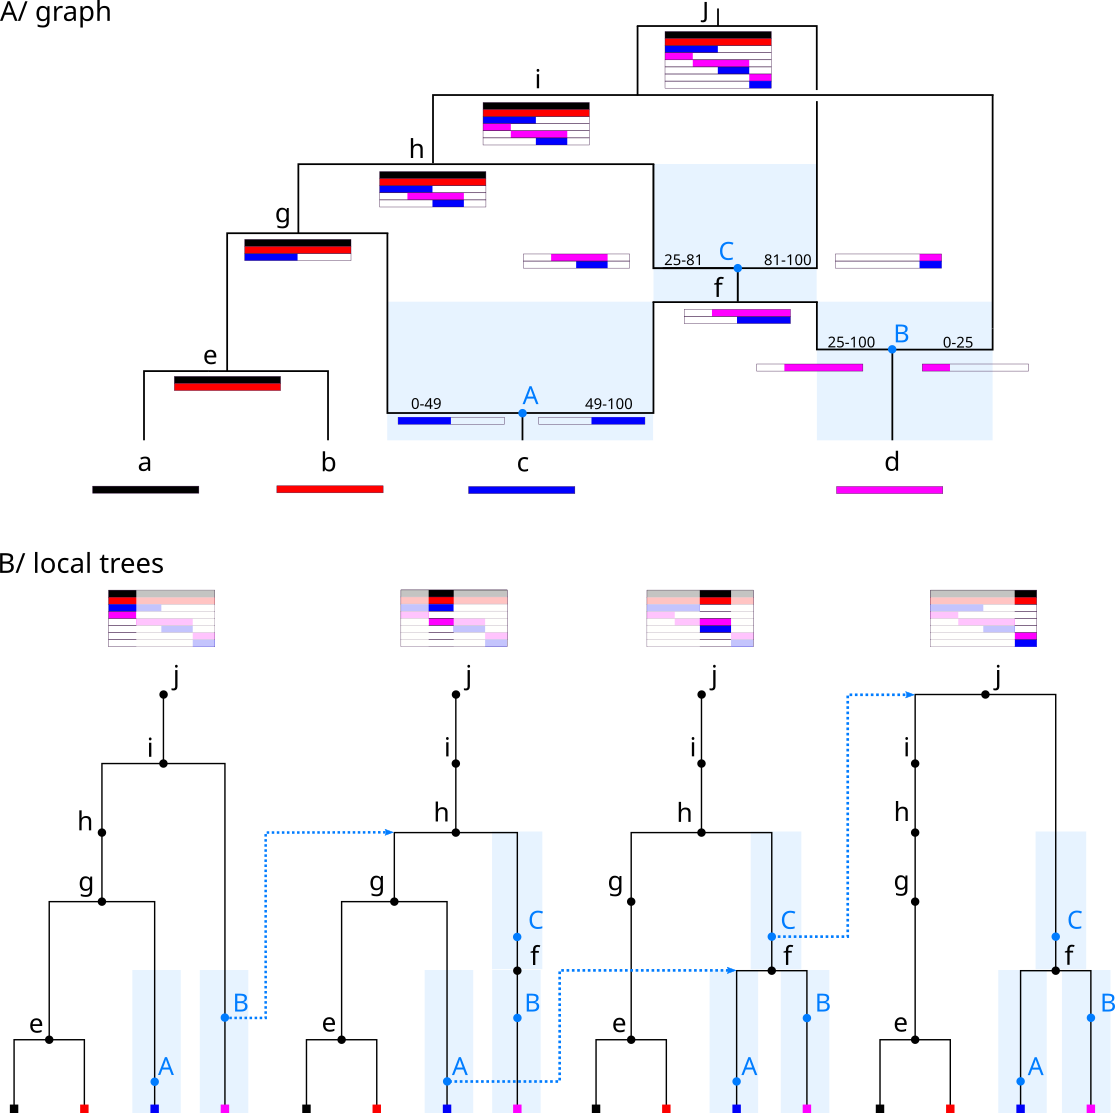
\includegraphics[width=0.9\textwidth]{figures/smc_custom_2rows_area_full_hap.png}
\caption{An ARG generated under the SMC, represented as a graph (top) and as a
series of local trees (bottom). To ensure the one-to-one correspondence
between both representations a node is recorded for each local tree whenever
a node is encountered along its ancestry path in the graph representation.
This results in nodes that (locally) have only a single child, and are therefore
(locally) unary. 
Nodes A, B and C are recombinants, i.e, have two parents in the graph
and are unary in the local trees. The blue shaded regions indicate
the range of possible times associated with these recombinants.
The blue arrows show the
standard left-to-right logic of the SMC whereby
the floating lineage coalesces randomly
with a the remaining portion of the local tree following recombination.
% By removing recombinant nodes, we limit the information on the time to each
% of these events to the windows (blue shaded array) delimited by the age of
% the child node and the minimum age of its parents.
}
\label{fig:smc-unary}
\end{figure}

An ARG can therefore be thought of either as a collection of inheritance
relationships between ancestral haplotypes,
or as a sequence of genealogical trees that have common node labels.
Fig.\ref{fig:smc-unary} shows a small ARG
that describes relationships between four samples on a 100bp piece of genome,
represented as both a graph (top) and a series of local trees (bottom).
Both structures represent the same information:
for instance, the fact that the ancestral genome at $A$
inherited the left half of its genome from ancestor $g$
and the right half from ancestor $f$
is seen in the fact that the first two trees have $A$ below $g$,
and the remaining have $A$ below $f$.
The blue dotted line from $A$ in the second tree to $f$ in the third tree
draws our attention to the fact that
the path traced by $A$'s ancestry switches at that point.
In fact, $A$ is in blue because it is a \emph{recombinant} node --
an ancestor that has a segment of genome inherited by a sample,
but that segment was inherited in two pieces from their parent.
Other nodes (labeled by black numbers) are either samples
or \emph{common ancestry} nodes --
ancestors that are the most recent common ancestor for two 
or more samples
at some place along the genome.

Crucial for the equivalence between the two representations is the presence of
nodes that only have a single child along one or more local trees --
i.e., are \emph{locally unary}~\citep{wong_general_2023}.
Recombinant nodes (in blue) have a single child in all trees.
However, common ancestry nodes can be locally unary as well:
for instance, sample $d$ inherited a longer stretch of genome from ancestor $f$
than sample $c$.
In the top plot, this is visible because the pink bar below node $f$
extends further to the left than does the blue bar,
while in the bottom plot, this is visible because node $f$ is parent to $d$
in the second tree, but not to node $c$, and so is unary.

%% Noved this section to section on smc
% A key observation of \citet{mcvean_approximating_2005}
% was that the sequence of trees along the genome
% generated by the SMC was Markovian \emph{after removing all unary nodes}.
% In other words, if we remove recombinant nodes entirely,
% and erase the unary portions of coalescent nodes,
% then the distribution of the next tree can be generated only knowing the current tree.
% (To see that the unary nodes makes the process non-Markov,
% consider that a node in a tree might be unary either because it's about to be a coalescent node
% or it already has been:
% looking at the second tree (Fig.\ref{fig:smc-unary}), we know node 5 will be coalescent further down the sequence
% because it was not present in the first tree.
% So, the first tree gives us information about subsequent trees
% that the second tree alone could not.)
% However, removing these unary portions of nodes seems odd
% when one considers the consequences of the inheritance paths through the
% ARG in the top figure.
% As pictured, both figures tell us that
% 3 inherits the middle bit of the genome from 7 through 5.
% However, if we erase 5 from the second tree,
% does this suggest that 3 inherited a single segment from 7 along two distinct paths?
% The graph-view of the ARG (above) makes it clear that this is unlikely:
% it is in fact reasonable to leave in these unary sections.

These locally unary nodes enable
us to uniquely identify all lineages that were hit by a recombination event,
even if we simplify 
the ARG by removing all recombinant nodes
($A$, $B$, and $C$ in Fig.\ref{fig:smc-unary}).
In the absence of these recombinant nodes, a recombination can be observed
easily enough as a change in parent going from one genomic region to the next.
Without the recombinant nodes we no longer know the precise time of each recombination event,
but we do still have constraints on it;
for instance, we know that $C$ happened somewhere between node $f$ and node $h$.
More generally, a recombinant node must happen somewhere between the child node
and the most recent of the parent nodes.
This is again easier to visualise using the
graph representation (blue shaded area, Fig.\ref{fig:smc-unary}).
Although these unary nodes are useful and to some degree clearly inferrable,
they are not always represented by simulators or ARG inference methods.
However, to our understanding this is because
the field is used to thinking in terms of the trees
rather than in terms of relationships between haplotypes,
not because of any question of knowability.
% JK I think we can but this out without-loss now given Halley's paper?
% Currently,
% \argweaver{} \citep{rasmussen_genome-wide_2014},
% \tsinfer{} \citep{kelleher_inferring_2019},
% \kwarg{} \citep{ignatieva_kwarg_2021}, and
% \texttt{SINGER} \citep{deng_robust_2024} estimate ARGs 
% including unary portions of coalescence nodes.
% However, it is unclear to what degree these are well-inferred,
% as most evaluation of inferred ARGs thus far has focused on marginal trees
% (e.g., \citet{brandt2022evaluation, kelleher_inferring_2019},
% but see \citet{deng2021distribution})
% and thus completely ignore such unary nodes
% (and their implications for inherited haplotypes).
See~\cite{fritze2024forest} for more discussion on unary nodes
and haplotype aware ARG comparison metrics.

% % % % % % % % % % % % % % % % % %
\subsection*{SMC backwards-in-time}\label{par:description}

% coalescent introduction: backwards-in-time
% left-to-right: Wiuf-Hein (difficult)
% SMC: although easy to reason about left-to-right sense
% 
The coalescent process describes the ancestry of a set of sampled genomes.
The original algorithm 
to simulate the coalescent with
recombination was formulated backwards in time
by Hudson \citeyearpar{hudson_properties_1983}. 
Wiuf and Hein later described
a tree-by-tree method to simulate the same stochastic process 
\citep{wiuf_recombination_1999}.
This along-the-genome approach is considerably more complex as the next 
tree to be simulated depends on all previous trees.
This idea however provided the basis of the 
SMC \citep{mcvean_approximating_2005}, restricting the set of all state
space transitions possible under the Hudson coalescent to
obtain a process that is Markovian both backwards-in-time, 
as well as along-the-genome.
In its backwards-in-time formulation, the SMC only requires a
simple modification to the coalescent with recombination.
Instead of allowing any pair of lineages to coalesce,
the SMC is the process in which only lineages with \emph{overlapping} 
genomic intervals may coalesce. The SMC' is a refinement 
of the SMC which also allows lineages with abutting genomic intervals to 
coalesce~\citep{marjoram_fast_2006}.
Although \citet{mcvean_approximating_2005} verbally described the SMC
using this backwards-in-time description, their analysis
was almost entirely in left-to-right terms,
and subsequent papers followed this trend
\citep{li_inference_2011,paul_accurate_2011,schiffels_inferring_2014,
rasmussen_genome-wide_2014}.

Linking the resulting tree-valued process along the genome back to
the relationship between the ``graph'' and
``local trees'' representation of ARGs, 
the Markovian property can be formulated as follows.
The distribution of the next tree within the series
of local trees can be generated only knowing the current tree,
provided that we remove recombinant nodes entirely,
and erase the unary portions of coalescent nodes.
To see that the locally unary nodes make the process non-Markov,
consider that a node in a tree might be unary either because
it's \emph{about to be} (in the left-to-right sense) a coalescent node 
or it \emph{already has been}:
looking at the second tree in Fig.\ref{fig:smc-unary},
we know node $f$ will be coalescent further along the sequence
because it was not present in the first tree.
So, the first tree gives us information about subsequent trees
that the second tree alone could not.
Further note that by limiting common ancestry events to overlapping 
pairs of lineages, we are guaranteed that all nodes in the ARG 
only carry ancestral material, that is,
genetic material that is inherited by either one of a set of samples
\citep{wiuf_ancestry_1999}.
We therefore require a single half-open interval to describe
the ancestral
material associated with each node in the ARG.

We now define the process more formally, by reintroducing
the notation of \citet{mcvean_approximating_2005} required to describe
the likelihood computation. This section
does not deviate from the original description of the SMC apart from
how coalescable pairs are counted. This subtle nuance
greatly simplifies the ability to keep track of coalescable pairs going
backwards in time.
At any point in time, the state of the process is 
the set of labeled lineages extant at time $t$,
$L(t) = \{X_j(t)\}$.
A lineage $X_j(t) = [x_{j}, y_{j})$ is labeled by 
an integer $j$ and defines the 
half-open genomic interval of its ancestral material.
% Ea
% where each lineage $X_j(t)$ is labeled by an integer $j$
% and represented by a 
% ancestral material. 
% Any lineage can thus be summarized as 
% for some interval endpoints $x_{j} < y_{j}$.
Because we look backwards in time, $t=0$ is today, and 
$L(0)$ consists of $n$ sampled lineages, labelled $0$ to $n-1$,
each represented by a single interval spanning the entire genome.
Then, the process evolves by a succession of common ancestor and recombination
events until each segment of ancestral material is only present in one lineage.
The waiting time to next event is determined by these two competing processes
with exponentially distributed waiting times as outlined below.

Recombination is described by a Poisson process of rate $r$ per unit 
of genomic length and time:
so, if $T(t) = \sum_j |X_j(t)|$ is total length of ancestral material
carried by lineages at time $t$,
then recombination occurs at instantaneous rate $rT(t)$.
A recombination to the left of $x$
(i.e., between base pairs $x$ and $x-1$)
with $x_{j} < x <y_{j}$ splits lineage $j$ into two new lineages,
given new, unique labels. We then remove lineage $j$
and add the two new lineages to the state $L(t)$.
This operation keeps the total amount of ancestral material unchanged.

Assuming a randomly mating, diploid population of constant size $N_e$,
common ancestry occurs between
two \emph{overlapping} lineages at rate $\lambda = 1/(2N_e)$.
Here we deviate from the McVean and Cardin formulation,
and define a strict total order on all lineages in $L(t)$:
for each lineage $X_j(t) = [x_{j}, y_{j})$ we define its 
order by the left coordinate $x_j$ and label $j$ (to break ties).
The instantaneous rate of coalescence then equals $\lambda$ 
multiplied by the number of overlapping pairs,
i.e., $\lambda \sum_{i \neq j} I_{jk}$,
where
\begin{equation} \label{def:coal}
I_{jk} = \begin{cases}
    1 & X_j > X_k \text{ and } x_j < y_k \\
    0 & \text{otherwise.}
\end{cases}
\end{equation}
We say that lineage $k$ can coalesce \emph{into} lineage $j$ if $I_{jk} = 1$.
Note that since $X_j > X_k$ implies that $x_j \ge x_k$,
this condition implies that the left endpoint $x_j$ of $X_j$
falls in the interval defined by $X_k$.
From the definition of the strict total order it follows that if $I_{jk} = 1$
then $I_{kj} = 0$. 
The newly formed lineage acquires the union of both intervals,
the original lineages are removed, and $L(t)$ is updated accordingly.
% [JK notes: need to explain here that this deliberately introduced 
% asymmetry doesn't affect the actual process. Also need to comment on 
% how the process terminates. Basically has the same subtleties as McVean and 
% Cardin, and not important for our purposes.]
For later use, also define $C_j(t)$ to be the set of
lineages that can coalesce into lineage $j$, i.e., 
$C_j(t) = \{X_k \in L(t) | I_{jk}(t) = 1\}$; 
thus, $|C_j(t)| = I_{j}(t) = \sum_{k} I_{jk}(t)$,
and the total rate of coalescence at time $t$ is $\sum_{j} |C_j(t)|$. 
Because $I_{jk}$ is defined in terms of a total order, the sets $C_j(t)$ are disjoint,
which will simplify likelihood computations later. In particular, although
recombination affects \emph{which} lineages can coalesce into $j$, it does not
change the \emph{number} of such lineages: in other words, a recombination
event changes $C_j(t)$ but not $I_{j}(t)$.

%% I have updated the description of the process below to avoid having to
% define yet another symbol.
%Another useful quantity to know is the number of lineages carrying material
%at each point on the genome:
%for a location $z$ and time $t$, this is
%\begin{equation}
%    N(t,z) = \vert\{j : z \in X_j(t) \} \vert
%\end{equation}

% [Do we need to get into this above-the-root subtelty here?]
% To ensure that the ancestral material carried by a single lineage can at
% all time be represented by a single half-open interval, we only update the
% endpoints of the involved lineages following common ancestry or recombination events
% such that only the minimal half-open interval whose endpoints have not fully coalesced
% is used to update $L(t)$. Note that empty intervals are not added to the state.
% %By reasoning about the process in this way we can keep representing 
% % all lineages by means of a single half-open interval until $\vert L(t) \vert = 0$
% % and the process terminates.

% %After any coalescence or recombination event,
% %the segment(s) $[x_j,y_j)$ (and $[x_k, y_k]$) carried by the involved lineage(s)
% %are replaced by a single segment $[x, y)$ whose endpoints have not fully
% %coalesced, i.e., $x = \min\{ z \ge \min(x_j, x_k) : N(t,z) > 1\}$,
% %and $y = \sup\{ z \le max(y_j, y_k) : N(t,z) > 1\}$. Note that empty intervals
% %are not added back to $L(t)$.

% Finally, by describing the SMC
% backwards in time, some intervals contained within the half-open
% interval representing a lineage might have fully coalesced before all the genetic
% material carried by that lineage has. As noted by \citet{mcvean_approximating_2005},
% such intervals can be observed as the stalks on the marginal genealogies (e.g., marginal trees
% for $[25, 81)$ Fig. \ref{fig:smc-unary}). Recombination events occurring within these smaller
% intervals however do not affect the marginal genealogies.

%The process of recombination and common ancestry events continues 
%Finally, there is one more operation that allows the process to terminate:
%portions of the edges of lineages that have entirely coalesced
%(i.e., that are ancestral to all samples) are removed.

%Formally, after any coalescence or recombination event,
%the segment $[x,y)$ carried by the lineage
%is replaced by the largest (pair of) segment(s) whose endpoints have not
%coalesced, i.e., $x$ is replaced by $\min\{ z \ge x : N(t,z) > 1\}$,
%and $y$ is replaced by $\sup\{ z \le y : N(t,z) > 1\}$.
%By reasoning about the process in this way we can keep representing 
%all lineages by means of a single half-open interval throughout.

%%%%%%%%%%%%%%%%%%%%%%%%%%%%%%%%%%%%%%
\subsection*{ARG likelihood} \label{par:liks}
We have defined the SMC process in terms of rates of various types of events.
In general, the likelihood for a continuous-time Markov process specified in this way
is $\exp(-\Lambda) \prod_i \lambda_i$,
where $\lambda_i$ is the rate of the $i^\text{th}$ realized event,
and $\Lambda$ is the sum of all rates of all possible events
integrated over the entire process
(also called the ``total hazard''). 
As discussed in the Introduction, in many cases these events are not what is 
estimated by inference methods, which produce, more fundamentally, a collection
of genetic inheritance relationships (edges) between ancestral haplotypes (nodes).
Our goal, therefore, is to decompose the overall likelihood into the
per-node and edge contributions, allowing us to compute likelihoods
for the incomplete ancestries estimated by current methods.
% Feel like we need a single sentence here that ties the first and second paragraph together
Using the out- and in-degree of the nodes we'll first reason about the number 
of common ancestor events and recombination events that could have resulted in 
the observed ARG. Next the information contained in the edges is leveraged to 
compute the total hazard associated with both types of events.
% , as well as graceful degradation in the presence of incomplete information.

%\comment{if we want to spell it out even further:
%Note that the time to the next event is distributed as $\Lambda \exp(-\Lambda)$. And
%the probablility that the next event is of type $i$ is $\lambda_i / \Lambda$.}

%where each edge $e$ is of the form $e = (p,c,x,y)$.
%Recall that this means that node $c$ inherited genetic material from node $p$
%over a region with span from $x$ to $y$ along the genome
%(see Figure~\ref{fig:likelihood}).
%So, $x$ and $y$ are genomic coordinates,
%while $c$ and $p$ are in $N$ (i.e., distinct sampled or ancestral haplotypes).

%Because the process of recombination only affects one lineage at a time
%(and does not even depend on the state of other lineages).
%On the other hand, common  events necessarily involve more than one lineage.
%However, the asymmetric way we define common ancestry events above
%allows us to uniquely associate each event with a single lineage,
%which allows us to cleanly factor the likelihood across edges and nodes.
% latter realized events, factor hazard across the edges.

% The structure of the ARG, as a collection of \emph{edges} $E$ and \emph{nodes} $N$,
% as well as the definition of both recombination and common ancestry events, allows us
% to cleanly factor the likelihood of the ARG across its edges and nodes.
% Not only does recombination
% naturally only affect one lineage at a time without even depending
% on the state of other lineages. Common ancestry events can be equally
% associated with a single edge given definition \eqref{def:coal}.
% The next paragraphs detail precisely how the number and the nature of the realized events
% can be determined based on the number of
% parents and children of each of the nodes in $N$ as well as how the total hazard can be
% factorized into the individual contributions of each of the edges.

Let $\deg_o(u) = \vert\{e \in E : p_e=u\}\vert$ be the out-degree of a node $u$,
i.e., the number of edges having $u$ as a parent.
Because mergers are binary in the SMC,
this must have been the result of $\deg(u) - 1$ common ancestry events,
and so this contributes a factor of $\lambda^{\deg_o(u)-1}$ to the likelihood
for nodes with any children.
Note however that this description is general and holds for the case of
more-than-binary mergers. By treating such polytomies as if there were zero-length edges
between a sequence of mergers, the order of these unresolved mergers does 
not affect the likelihood. Under the SMC the likelihood of a zero-length edge is zero.
This is not special: since edge lengths are continuously distributed,
the likelihood of any particular value is also zero.

Similarly,
let $\deg_i(u) = \vert\{e \in E : c_e=u\}\vert$ be the in-degree of a node $u$,
i.e., the number of edges having $u$ as a child.
Each additional edge that is ancestral to a given node
implies one additional ancestral recombination event,
and thus a factor of  $r^{\deg_i(u)-1}$ in the likelihood,
if the node has any parents.
Put together, these two contribute
\begin{equation}\label{eq:coal}
    \prod_{u \in N} \lambda^{\deg_o(u)-1} r^{\deg_i(u)-1}  
    =
    r^{|E|-|N|+n_r} 
    \lambda^{|E|-|N|+n_s} 
\end{equation}
to the likelihood,
where $n_r$ is the number of nodes with in-degree 0 (roots),
and $n_s$ is the number of nodes with out-degree 0 (usually, samples).
(The simple form follows because each edge contributes exactly one
to some node's out-degree and some node's in-degree.)


\begin{figure}
    \centering
    \includegraphics[width=0.65\textwidth]{figures/single_event.png}
    \caption{
    Graphical representation of the events associated with the edge $(p,c,x,y)$.
    The lineage carried by $c$ (dark green bar) spans $[x_c,y)$ 
    until a recombination event (blue
    dotted line) splits it into two segments. Left and right hand segments coalesce
    (with the pink and yellow lineages, respectively)
    at times $t_{p'}$ and $t_p$ respectively, bounding the time to recombination by
    % JK used to be: $(c. \min(t_p, t_{p'})$
    $\min(t_p, t_{p'})$.
    % JK: not sure this helps? 
    % Note that the contribution to the recombination hazard
    % by edge $(p,c,x,y)$ only covers ``half'' of the green shaded area. The other
    % half is contributed by edge $(p', c, x_c, x)$. 
    \label{fig:likelihood}
    }
\end{figure}

Now consider the ``hazard'' associated with recombination.
Begin with an edge $e = (p,c,x,y)$.
This implies that there was a sequence of lineages
from the time of the child $c$ (call this time $t_c$)
back to the time of the parent $p$ (again, $t_p$),
that contained the segment $[x,y)$,
and the lineage that directly inherited from $p$
had the segment $[x,y)$ (see Fig.~\ref{fig:likelihood}).
We therefore know there was no recombination between $x$ and $y$
on any of those lineages 
over this time span,
the probability of which is
$\exp(-r \mathcal{A}_e)$, where $r$ is the recombination rate
and $\mathcal{A}_e$ is the total area (eligible links multiplied by length in time) of the edge.
The length in time of the edge is just $t_p - t_c$,
while the number of ``eleigible links'' in the edge is the number of adjacent base pairs in the edge
on which recombination did not occur, which is either $y-x$
(if this edge is the leftmost of all edges above node $c$)
or $y-x-1$ (otherwise).
So, the first contribution to the likelihood from this edge $e$ is
\begin{equation}\label{eq:span}
A_e(r) = \exp(-r (y-x - \mathbbm{1}_{x > x_c})(t_p - t_{c})) ,
\end{equation}
where as for lineages, $x_c$ is the leftmost position of the edges whose children are $c$.
% Note that if a recombination did occur, then the number of links not
% affected by recombination is 1 less (see eq.~\eqref{eq:depth}).

Finally, we turn to the hazard associated with common ancestry events.
To do this,
we need only consider what happens along the left side of each edge.
Following what we did for lineages, we define a total order on edges
by ordering by left endpoint and breaking ties by child
(i.e., $(p,c,x,y) < (p',c',x',y')$
if $x<x'$, or if $x=x'$ and $c<c'$).
The instantaneous rate of coalescence of a lineage whose left endpoint is at $x$
at a given time is equal to $\lambda$ multiplied
by the number of earlier lineages that overlap $x$ at that time.
Using this total order, we can define
$I_e(t)$ to be the total number of earlier edges that overlap edge $e$
and are present at time $t$.
Then, the cumulative hazard for common ancestry events of edge $e$
between time $s$ and $t$ is given by $F(e, s, t) = \int_{s}^{t} I_{e}(z) dz$.
If the edge $e = (p,c,x,y)$
is the leftmost segment of material inherited by node $c$
(e.g., the left hand segment ancestral to node $c$
in Fig.~\ref{fig:likelihood}),
then no recombination occurred along this edge and 
this edge simply contributes $\exp(-F(e,t_c,t_p))$ to the likelihood.
However, if the edge is \emph{not} the leftmost segment
(as shown in Fig.~\ref{fig:likelihood}),
then it was initiated by a new recombination breakpoint,
and we need to integrate over possible times the breakpoint occurred.
If this is the case, there is another edge $(p',c,x',x)$ with the same child node,
immediately adjacent to the focal edge $(p,c,x,y)$.
The recombination event that split the two must have happened between $t_c$
and the smaller of $t_p$ and $t_{p'}$.
Taking all this into consideration,
the contribution to the likelihood here is
\begin{equation}\label{eq:depth}
B_e(r, \lambda) = \begin{cases}
    e^{-\lambda F(e, t_c, t_p)}
        & \qquad \text{if } x=x_{c} \\
    \int_{t_c}^{t_{p} \wedge t_{p'}} e^{- r s} e^{-\lambda F(e, s, t_{p})} ds
        & \qquad \text{if } x>x_{c} .
\end{cases}
\end{equation}
% In that case $x=x_{c0}$ and $c$ did not coalesce until $t_p$.
% Alternatively, $x$ can be a new recombination break point that
% occurred on the lineage represented by $c$ at some time $s$ between $t_{c}$
% and $\min(t_p, t_{p^{\prime}})$, where $p^{\prime}$ is the parent of the
% edge $(c, p^{\prime}, X_{cp^{\prime}})$ ending at $x$. The new lineage formed
% by the recombination event and starting at $x$ can be given a temporary label
% $c_s$. In both cases, the cumulative hazard of a lineage $a$ coalescing
% between time $s$ and $t$ is given by $F(c, s, t) = \int_{s}^{t} I_{c}(u)du$
% such that:
%\comment{This is the old equation; I think the $e^{-rs}$ should not be there,
%    since it's already taken into account by \eqref{eq:span}.
%    Plus, the $\lambda$ and $r$ factors are now elsewhere.}
%\begin{equation}\label{eq:depth_old}
%B_{(c, p)}(\theta) = \begin{cases}
%e^{-\lambda F(c, t_c, t_p)} \lambda^{I_{cd}(t_p)} & x=x_{c0} \\
%\int_{t_c}^{t_{p} \wedge t_{p^{\prime}}} r e^{-rs} e^{-\lambda F(c_s, s, t_{p})} ds \lambda^{I_{c_{s}d}(t_p)} & x=x_{c_{s}0}>x_{c0} \\
%\end{cases}
%\end{equation}
%\comment{Do we still need this bit?}
%Here, the (second) exponential term gives the probability of not observing a
%coalescence event before $t_p$. In case of a recombination, $re^{-rs}$ further
%gives the probability of observing a recombination
%at time $s$ given a Poisson process along position $x$ with rate $r$.
%The time of the recombination is integrated out.
%The last term gives the point probability density of the coalescence event
%that terminates the edge. The indicator function is used to resolve
%the non-reciprocal nature of coalescence events as defined in \ref{def:coal}.
The overall likelihood of an ARG $\mathcal{G}$ defined by the set of edges $E$ and nodes $N$
given parameters $\theta$ is then given by
\begin{equation}\label{eq:full-lik}
    \mathcal{L}(\mathcal{G}|r, \lambda)
    =
    (r)^{|E|-|N|+n_r} (\lambda)^{|E|-|N|+n_s} \prod_{e \in E} A_e(r) B_e(r, \lambda) .
\end{equation}
One significant advantage of this formulation is that the computation time
is linear in the number of edges, and an efficient algorithm exists
to keep track of $I_e(t)$ (see Appendix).
% Although the first two factors are easily expressed in terms of numbers of edges and nodes,
% we will see below
% that in practice it is convenient to absorb these terms into per-edge contributions.
% We can also accommodate stepwise changes in the 
% coalescence rate (or recombination rate)
% through time by intersecting the internode intervals with the rate change
% intervals; rate changes along the genome can be incorporated similarly.
Note that we have only considered the topology and branch length information here
and not considered mutational information. 
Assuming the infinite sites model, computing the likelihood of 
an ARG given a mutation rate $\mu$ and set of mutations is straightforward, 
as the overall likelihood can be directly decomposed into the per-edge
contributions~\citep{baumdicker_efficient_2021,mahmoudi_bayesian_2022}.

% The likelihood of a set of mutations given an ARG $\mathcal{G}$ given mutation rate $\mu$ is
% \begin{equation}\label{eq:lik-mut}
%     \mathcal{L}(\mathcal{D}|\mathcal{G}, \mu)
%     =
%     \prod_{e \in E} \frac{(\mu(t_p-t_c)(y-x))^{m_e}}{m_e!} e^{-\mu (t_p-t_c)(y-x)} ,
%     % I don't think the following is correct:
%     % \frac{1}{\mathcal{M}!} \prod_{(p, c, x, y) \in E} e^{-(y-x)(t_p-t_c)\mu^{|m_e|}}
% \end{equation}
% where 
% % $\mathcal{M}$ the total number of mutations and 
% $m_e$ is the number of mutations along edge $e$ 
% and as before $e = (p,c,x,y)$
% \citep{mahmoudi_bayesian_2022}.

% % % % % % % % % % % % % % % % % %
\subsection*{Robustness to partial and incorrect information}
Eq.~\eqref{eq:full-lik} allows us to compute a likelihood for \emph{any}
collection of nodes (ancestral haplotypes that lived at some time 
$t$ in the past) and edges (a record that child node $c$ 
inherited the genomic interval $[x, y)$ from parent node $p$)
under the SMC. Other than some basic consistency constraints (e.g., parents
must be older than children) there are no requirements on the topology
described, and in particular, no requirement that the events from the 
model (the SMC) should be explicitly identified in the graph. Our 
formulation reasons about the events that \emph{could have resulted in}
the observed nodes and edges, and therefore frees us from the requirement
of having to explicitly write those down. In this section we 
illustrate the robustness
of this approach to incomplete and potentially incorrect
information about recombination and 
coalescent events via a proof-of-concept example. 
% in which we 
% remove various levels of detail from a simulated ARG.

\begin{figure}
    \centering
    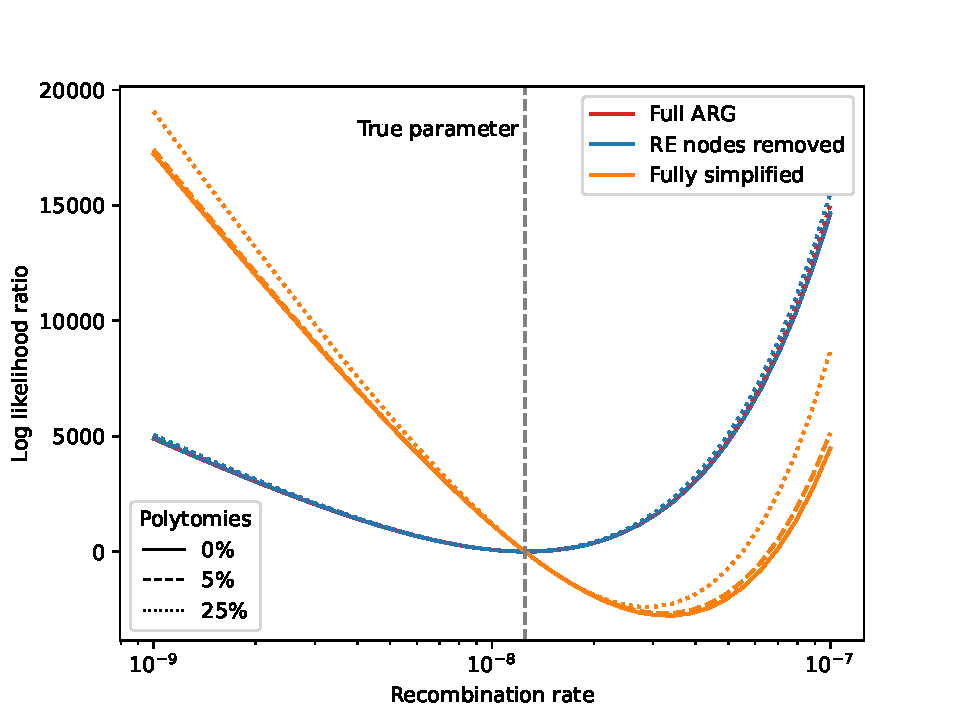
\includegraphics[width=0.8\textwidth]{figures/likelihood_surface}
    \caption{Log likelihood-ratio curves for ARGs with various properties.
    The ``Full ARG'' here is the result of an 
    msprime simulation of the SMC (100 diploid samples, genome length 1Mb, 
    $r=\mu=2.5\times10^{-8}$, $N_e=1\times10^4$).
    The ``RE nodes removed'' ARG is the 
    result of simplifying out all of the recombination nodes,
    and the ``Fully simplified'' ARG has all locally unary nodes removed. 
    Each of these simulated ARGs additionally has 5\% and 25\% of the 
    internal nodes removed to create polytomies.
    We also show the results for ARGs inferred from the original simulation
    data using tsinfer and tsdate 
    (see text for details), in which we use the default output of tsinfer
    including unary nodes (tsinfer+tsdate), and in which we fully simplify 
    before passing to tsdate (tsinfer+tsdate FS). 
    See the text for details on how the likelihood ratio 
    values are computed.
    The ``Full ARG'' and ``RE nodes removed'' lines coincide.
    \label{fig:lik-surface}}
\end{figure}

In Fig~\ref{fig:lik-surface} we begin with a realisation of the SMC 
containing complete information about every simulated event
(Full ARG; 9,378 nodes; 13,221 edges; 2,933 trees). 
We then plot the likelihood computed by Eq.~\eqref{eq:full-lik} 
as we vary the recombination rate parameter $r$, as a ratio
of the likelihood at the true value of $r$. 
Reassuringly, we can
see that the minimum of the likelihood-ratio curve when using the 
full simulated ARG is close to the true value of the parameter.
(The likelihood ratio curve obtained when computing the likelihood
under the full coalescent with recombination model using the KYF
formula is identical; not shown.)
We next compute the likelihood ratio for the ARG obtained when we 
simplify out the recombination nodes from the full ARG
(RE nodes removed; 3,332 nodes; 6,901 edges; 2,933 trees; note that msprime 
uses distinct nodes for the left and right parent of each recombination).
The curve we obtain is indistinguishable from that of the full
ARG, demonstrating that the locally unary portions of coalescent nodes 
contain all the information that we need about recombination events
for this application.
When we fully simplify the simulated ARG
to remove all locally unary nodes from trees 
(Fully simplified; 3,332 nodes; 10,674 edges, 2,933 trees) 
we can see there is a significant loss of information,
and the minimum of the 
likelihood ratio surface is biased away from its true value.
(See~\cite{wong_general_2023} for more discussion on varying 
degrees of ARG simplification.)

Fig~\ref{fig:lik-surface} shows that Eq.~\eqref{eq:full-lik} is also remarkably
robust to the presences of polytomies in this example. For each of the three
ARGs discussed in the previous paragraph, we also evaluated the likelihood
for ARGs in which 5\% or 25\% of the internal ARG nodes are removed and 
edges adjusted accordingly.
This introduces polytomies at varying degrees in the different ARGs because 
deleting a node in a tree (and connecting its children directly to its
parent) will only create a polytomy if the parent 
is not unary. Thus, while deleting 25\% of the internal nodes 
in the fully simplified ARG created an average of 33 polytomies
over the 2,933 trees along the sequence (each tree having 
200 leaf nodes), it resulted in an average of 21 polytomies
per tree in the ARG where recombination nodes have been removed,
and only 10 in the full ARG (which has an average of 1026 unary 
nodes per tree).
%     name                  leaves  unary       binary  poly
% 0   full_arg_smc          200.0   1094.417661 199.000000  0.000000
% 1   unary_coal            200.0   456.396522  199.000000  0.000000
% 2   fully_simplified      200.0   0.000000    199.000000  0.000000
% 3   tsinfer_tsdate        200.0   192.447590  119.754399  32.270849
% 4   tsinfer_fs_tsdate     200.0   0.000000    119.563898  32.322684
% 5   py_full_arg_smc_0.05  200.0   1025.565973 192.662462  3.153086
% 6   py_unary_coal_0.05    200.0   429.315017  190.182253  4.372696
% 7   py_fully_simied_0.05  200.0   0.000000    185.691468  6.393174
% 8   py_full_arg_smc_0.25  200.0   779.846233  176.830549  10.307876
% 9   py_unary_coal_0.25    200.0   323.054926  154.422588  21.104016
% 10  py_fully_simied_0.25  200.0   0.000000    117.096174  33.241986
Given this disparity in the number of polytomies introduced, the 
effects on the likelihood across the three examples are not entirely
comparable. For the ARGs containing unary nodes, 
removing 25\% of the internal 
nodes has negligible effect, and even on the fully simplified 
ARG has a very minor effect on location of the minimum.

Fig~\ref{fig:lik-surface} also shows results for ARGs inferred from the 
simulated data using tsinfer and tsdate~\citep{wohns_unified_2022},
using default parameters for tsinfer, and the true values of mutation
rate and $N_e$ for tsdate.
In the first, we use the default output of tsinfer 
(2,148 nodes; 5,589 edges; 1,307 trees; 3,039 mutations).
This ARG has an average of 192 unary nodes, 120 binary nodes, and 32 nodes
with three or more children per tree. Tsinfer does not directly estimate
recombination events; the breakpoints between trees are the consequence of
switches between parental haplotypes in the 
\cite{li2003modeling} copying process. Information about 
recombination events in the returned ARG is therefore quite imprecise,
and likely to contain incorrect and contradictory details if one were to 
attempt to reconstruct the exact subtree-prune-and-regraft 
moves~\citep[e.g.][]{rasmussen2023espalier}. Nonetheless, in
this toy example at least, our likelihood function performs well
on the output of tsinfer, with the minimum close to the true
parameter value. We also show the likelihood curve obtained when we 
fully simplify the output of tsinfer 
(1,865 nodes; 7,511 edges; 1,252 trees; 3,039 mutations)
before dating. We can see that, as with the true data,
removing all the unary nodes results in a significant bias
away from the true value of the recombination rate parameter.

\subsection*{Piecewise decomposition over time}
\begin{figure}
    \centering
    \includegraphics[width=0.8\textwidth]{figures/3-slices-whitespace.png}
    \caption{Simulated ARG under the Hudson coalescent (left). $N_e$ is constant
    for each of the 3 time slices:
    from 0 to 1,000 generations ago $N_e$ is 10,000;
    from 1,000 to 5,000 generations ago it is 5,000;
    and past that it is 10,000.
    Remaining parameters: genome length is 10kb, 20 diploid samples, and
    $r=2.5\times10^{-8}$. 
    There are 148 edges in the resulting ARG.
    A single $N_e$ value was estimated for each
    of the three slices of the ARG separated by
    the true population size change time points.
    The inferred posterior distribution (right) using the SMC-likelihood was
    obtained using a uniform prior. The number of edges per time slice
    (from most recent to oldest) was: 68, 57, and 23. Locally unary nodes were
    omitted for clarity.}
    \label{fig:3-arg-slices}
\end{figure}

Our final example explores decomposition of the likelihood
into separate components for different segments of time.
By explicitly associating a single likelihood with each edge,
we can compute the likelihood for any slice of the ARG taken in
time and/or along the genome.
In the case of a fully precise ARG, in which each recombination
event has an exact time,
this is true as long as the slicing operation does not erase the
information on whether an edge is associated with the left or
right hand segment generated by a recombination event. In the absence
of the exact time to recombination, the integral in
Eq.~\eqref{eq:depth} means that the likelihood
for the entire ARG does not factorize into the likelihoods of these
individual slices. More precisely, the likelihood associated with any
edge that is initiated by a recombination breakpoint cannot be factorized
into the product of two integrals of the same form.
However, as long as the individual slices of the ARG contain sufficient
information we can approximate the true integral as the product of the
integral of the slices. Fig.~\ref{fig:3-arg-slices} demonstrates this idea
on a toy example. We simulated an ARG under human-like parameters with
two effective population size changes, and subsequently computed the posterior
distribution on the three effective population sizes
using a uniform prior on each slice independently.
The result is reasonably accurate, despite only using 10kb of sequence.

% This approach therefore strengthens
% the inherent ability of ARGs to provide us with temporal
% resolution and context to a dataset of genetic variation.
% It also opens up the opportunity for more efficient optimization
% strategies during inference given that each slice of the ARG can be
% processed independently. 

% And it further highlights the flexibility
% of the algorithm. Simply stated and from a data structure perspective,
% we can compute a likelihood under the SMC for any valid tree sequence.
% The \texttt{tskit} library provides a wide range
% of subsetting operations on tree sequences allowing us to slice
% the ARG in time and/or space, as well as to reduce the number of
% tracked samples. Any such subset of the tree sequence is itself
% a valid tree sequence for which we can again compute a likelihood.

\section*{Discussion}
The key contribution of this paper is to rederive a classical
ARG likelihood function in a way that supports the sort of partial 
and imprecise information
provided by some modern ARG inference tools,
using a novel backwards-time derivation of the SMC.
The underlying process that we reason about probabilistically is still
composed of events affecting lineages, but, because we
do not necessarily observe or estimate these events,
we integrate over the possible timings implied by the information
in the input ARG.
Our method can compute a likelihood under the SMC for a very general class of 
ARG~\citep{wong_general_2023}, 
a significant increase in flexibility over the 
strict input requirements for the classical Kuhner-Yamato-Felsenstein 
formulation. 
Locally unary nodes play a key role, and although not
currently a common focus of ARG research~\citep{wong_general_2023}, 
they are estimated by tsinfer and can be imputed to high a
degree of accuracy from fully simplified ARGs~\citep{fritze2024forest}.
We have shown via some illustrative examples that the formulation is 
robust to incomplete and imprecise information, tolerating the loss 
of a significant fraction of the internal nodes in the ARG to minimal effect.
We have also shown that the likelihood function performs well 
(at least in our toy example) on ARGs inferred by tsinfer+tsdate,
successfully capturing information about latent recombination events
from imprecise and noisy data.
% I think we have to grasp this nettle or we're inviting the reviewers to 
% give us a bunch of "what if you tried this" bits of extra homework.
Theoretical explanations of this apparent robustness,
and fully characterising the properties of the likelihood on the output 
of tsinfer and other methods is an important avenue for future work.
Similarly, while there are many potential applications to concrete 
inferential problems, the details are nontrivial and must be
consigned to future work.

% Structural uncertainty
 
% A major advantage of our approach is that it does not require
% us to explicitly identify common ancestor and recombination events 
% in the input. Indeed, 
% we can compute a likelihood for any ARG in \texttt{tskit} format,
% potentially bridging the gap between population genetic theory and the 
% varied structures inferred by current methods~\citep{wong_general_2023}.

% there are some caveats. By treating each edge independently,
% our algorithm will still produce a value for ARGs with
% the various degrees of completeness to which inheritance
% is documented by the different ARG inference methods.
% % : e.g., polytomies, absence
% % of locally unary coalescence nodes, unpreserved identify of internal nodes
% % across local trees, etc.
% % However, many of these imprecisions violate the implicit
% % assumptions of the likelihood computation.
% For example, we assume the 
% presence of locally unary nodes to correctly identify the
% full extent of all lineages going back through time 
% and therefore recombination events, but this information
% may be incomplete (e.g., the full simplifed ARG in Fig.~\ref{fig:lik-surface})
% or even incorrect.
% % Without these unary nodes, our algorithm will detect a recombination
% % event along both coalescing lineages in case of a (sub)tree height changes along
% % the ARG as both edges would switch parent nodes. 
% Locally unary nodes are not a common aspect of current ARG 
% research~\citep{wong_general_2023}, but 
% are estimated by tsinfer, and can be imputed to high
% degree of accuracy from fully simplified ARGs~\citep{fritze2024forest}.
% Determining the effects of various forms of \emph{incorrect} topology on
% these likelihoods requires further research.

% [Something about polytomies]

Our results, while preliminary, suggest that ``full ARGs'', in which 
each recombination and common ancestor event is precisely estimated,
contain a significant degree of redundancy in terms of capturing 
information about the generative process. 
It is possible, therefore, that explicitly estimating 
\emph{all} such events is not necessary to sample ARGs under the 
SMC (as ARGweaver and SINGER do). 
A combined approach, in which the uncertainty around the
ordering of events that are 
weakly informed by the data is encoded structurally in the 
graph and other forms of uncertainty captured by sampling from 
the posterior, may yield further improvements in 
scalability for statistically rigorous inference.
% Signicant work would be needed, however, to make 
% downstream analysis robust to such stuctural uncertainty;
% polytomies, for example, are often not
Another exciting prospect for ARG inference is the development of 
``hybrid'' inference methods, where hueristic methods such as 
tsinfer or ARG-Needle are used to infer
the details of the recent past in huge datasets such as 
UK Biobank, passing over to a rigorous model-based
approach for the ancient past.
This is similar in spirit to the widely-used approach 
of simulating complex dynamics of the recent past using 
detailed but slow models and using faster coalescent simulations
in the distant past when the assumptions required 
are more justified~\citep{bhaskar_distortion_2014,
kelleher_efficient_2018,haller_tree_2018,nelson_accounting_2020}.
% Maybe we shouldn't bother saying this, but I can't resist the 
% opportunity to say "hey, you should be using tskit!"
% It feels like some PIs aren't getting this message, so need to have
% it spelled out.
Just as forward and backward simulations are useful in different contexts
and can be combined to great effect,
large-scale hueristic and Bayesian sampling inference methods have their 
applications, and there may be synergy in their combination. 
% This is pretty weak, tbh.
The practical details of ``handing over'' between methods
will require cooperation and precise communication;
the tskit library, with its well-defined data model and flexible
metadata support, is the ideal basis for this.


% This can be mitigated by limiting
% the number of `inferrable' recombination events per coalescence event to 1
% (see fig \ref{sup:fig:rec-correction}).
% \comment{I'm not editing this in since I'm not sure I've got it right:
% I think that as written, our algorithm would count an extra recombination
% and and extra coalescence for any edge that got split up by removing the unary bits.
% This could be corrected for in the algorithm, but it would require extra bookkeeping,
% and make the likelihood not so easily a product over edges. (?)}
% 
% \comment{this was previously part of the discussion, have grouped it here.}
% Although their presence is crucial to our ability to embed any local tree in the
% ARG, the concept and their importance are still relatively new (but see
% \citet{wong_general_2023}).
% We have briefly touched upon the observation that in
% the presence of unary nodes we seem to augment the left-to-right logic of the SMC
% with some additional information. Yet, we believe that the topic of locally
% unary nodes in general requires further exploration.
% And more specifically, we see it as future work to fully quantify to what
% extent the absence of these locally unary nodes will affect the shape of the
% likelihood surface given any set of parameters.

%%% remarks on precision of information + useage of likelihood to either
%%% estimate parameters (not goal here) or use as instrument to improve accuracy to infer ARGs


% [JK: this needs significant work]
% Here, we have introduced a scalable algorithm to compute likelihoods
% under the SMC for a general class of ARGs. By formulating the SMC backwards in time
% we were able to associate a single likelihood value with each edge in the ARG.
% The compatibility of the algorithm with the \texttt{tskit} library allows us to
% exploit its associated efficiencies both for the current work and its future
% applications. This work will contribute significantly
% to ARG-based analysis becoming a standard part of the population
% and statistical genetics toolkit.
% In particular, we see two main applications for the work presented here.
% Firstly, the ability to associate inferred ARGs with a likelihood given a demographic
% model and an associated set of parameters, will help bridge the gap between the tremendous recent
% advances in ARG inference and the current state of the art statistical inference of
% past demography.

% The second and probably the most important application of the ability to associate a more
% general class of ARGs to a principled model is the ability to boost the current efforts
% in ARG inference. 
% % great starting point for MCMC
% Any inferred ARG can be used a good starting point
% for a future MCMC-sampler. This potentially implies a massive runtime reduction by
% reducing the necessary burn-in period. Furthermore, by integrating out the exact time
% to the recombination event we further restrict the size of the ARG space that needs to
% be explored. This MCMC-sampler would again rely on the tree sequence data structure to
% efficiently generate and evaluate any new proposal (see \citep{mahmoudi_bayesian_2022}).
% % hybrid ARG-inference: scalability + bringing ARG down from pedigree dominated phase
% To further improve scalability, hybrid ARG-inference methods could be designed which
% rely on heuristic approaches to bring the ARG down from the initial pedigree-dominated phase,
% and subsequently use a principled approach to perform ARG inference for the second phase.
% This idea resembles the tried and tested approach of hybrid backwards-in-time simulations 
% that combine Wright-Fisher dynamics in the very recent past and coalescent simulations 
% for the remaining time \citep{bhaskar_distortion_2014, nelson_accounting_2020}. This hybrid
% approach has enabled large scale simulations while avoiding the documented biases of the
% coalescent relative to the Wright-Fisher model \citep{bhaskar_distortion_2014, wakeley_gene_2012}. 
% The same approach could be thus used for ARG-inference where one can rely on a heuristic 
% inference method for the recent past, while using a model-based approach beyond that cutoff point.

% Finally, acknowledging the uncertainty associated with ARG inference does not
% necessarily require a full-blown MCMC sampler. Instead, recognising those parts of
% the ARG for which we lack information for confident reconstruction and resolving
% them stochastically by sampling from the coalescent rather than completely arbitrarily
% would already be a major step forward. 

% % this part is only a very rough idea, might be better to leave it out if we can't make it more concrete.
% We believe that quantifying uncertainty does not have to be associated with sampling
% from the space of all compatible genealogies. Uncertainty could also
% be quantified and passed on as metadata to the nodes in the data format storing the ARG.

% [Note: a point to make here is that the idea of combining heuristic large-scale 
% inference with model based inference is analogous to the combination of 
% coalescent simulation and forwards time simulation. We can also draw lessons
% from developers of different methods cooperating and using the tskit library
% to enable this.]

% Additionally, there is a rich suite of tools growing around
% the \texttt{tskit} ARG library~\citep{ralph_efficiently_2020}
% including simulation~\citep{kelleher_efficient_2016,kelleher_efficient_2018,
% adrion_community_2020,terasaki_geonomics_2021,
% baumdicker_efficient_2021,
% korfmann_weak_2022, petr_slendr_2023,tagami_tstrait_2024},
% ARG inference~\citep{kelleher_inferring_2019,speidel_method_2019,
% wohns_unified_2022,mahmoudi_bayesian_2022,
% rasmussen_espalier_2022,
% zhang_biobank-scale_2023,zhan_towards_2023} and analysis
% packages
% % etc
% \citep{nowbandegani_extremely_2023,fan_likelihood_2023}.
%% NOTE: this is some orphan text from the intro that can be rejiggered for the 
% discussion. We can talk about precision of recombination estimates a bit 
% here I think, as it is an important topic.

% Both approaches have further formed the basis (of many) of the recent advancements in
% ARG inference methods \citep{rasmussen_genome-wide_2014, heine_bridging_2018,
% kelleher_inferring_2019, speidel_method_2019, rasmussen_espalier_2022, zhang_biobank-scale_2023}.
% A further classification of these methods could be made based on the level of detail
% that is provided on recombination events. The first real breakthrough in large-scale
% ARG inference, \argweaver, heads the first group.
% The ARGs sampled by \argweaver from the posterior distribution
% given the observed variational data, are all fully precise and detailed in the sense
% that all events are explicitly inferred. Note however that the set of possible node times
% has to be limited to enable the usage of an HMM. The other more recent methods, although
% still SMC-based, have added heuristic pre- and/or post-processing steps
% that have allowed them to extend their approach to larger sample sizes. We should also
% mention \kwarg and \texttt{ARGinfer} in this category of methods producing fully detailed ARGs
% although these are not based on the SMC or the copying algorithm. In fact they represent
% two extremes along the approximation continuum with \kwarg being entirely
% parsimony-based while \texttt{ARGinfer} is a CwR-based MCMC sampler.

%% Recent progress in ARGs through approximate structures}

% The second group of methods (\tsinfer, \relate, \argneedle) has marked a significant
% leap in scalability. These methods derive their scalability at least to a certain
% degree from the fact that the ARGs they infer are approximate structures. In particular,
% recombination is an emergent property of the inferred ARGs, explaining tree topology
% changes going from one local tree to the next. The recombination events themselves
% are not explicitly inferred and are thus not part of the resulting data structure.

% The computational gains from not having to pinpoint recombination events tie in
% with the inevitable uncertainty associated with ARG reconstruction [Hayman, 2022, ADD REFS].
% Some approaches have embraced the approximate nature of the resulting ARG by, for
% example, highlighting the inability to resolve certain splits and instead representing
% them as polytomies \citep{kelleher_inferring_2019}. Taken together this means that the
% degree of completeness in which genetic inheritance from ancestors to descendants is documented
% by each of these methods varies extensively.
% [TO ADD: these methods only provide point estimates]


\section{Data availability}

All scripts and data used for this manuscript are available at
\url{https://github.com/gertjanbisschop/smc-bit-paper},
and an implementation of the algorithm is available at
\url{https://github.com/gertjanbisschop/runsmc}.
\FloatBarrier
\bibliographystyle{abbrvnat}
\bibliography{paper.bib}

\setcounter{secnumdepth}{2} % Print out appendix section numbers

\section*{Appendix}
\appendix

\setcounter{table}{0}
\setcounter{figure}{0}
\renewcommand{\thetable}{A\arabic{table}}
\renewcommand{\thefigure}{A\arabic{figure}}

% % % % % % % % % % % % % % % % % %
\subsection*{Algorithm} \label{par:algo}
In this section we describe how to efficiently compute the likelihood under the SMC
from an ARG stored using the \texttt{tskit} tree sequence encoding. 
The tree sequence format encodes relationships using \emph{edges},
along with additional information that
allows us to sequentially recover (and reason about 
their differences) 
efficiently~\citep{kelleher_efficient_2016, ralph_efficiently_2020}.
The order of the edge deletions and insertions required to move from one local tree $T_1$ to
the next, $T_2$ imposes the strict total ordering on edges
(see definition~\eqref{def:coal})
that is needed to efficiently maintain the state of $I_e(t)$ for each focal edge $e$.
Indeed, following the removal of edges that do not persist in $T_2$,
we simply declare that each subsequently added edge
can only coalesce with the already-visited edges 
that make up the (partially) reconstructed local tree $T_2$.

\begin{figure}[!ht]
\centering
\includegraphics[width=\textwidth]{figures/ts_algo_2rows.png}
\caption{Likelihood computation algorithm. 
Moving along the genome we transition from
local tree $T_1$ to the next, $T_2$ in three steps. 
Edges that do not persist in $T_2$ are
removed first. Edges starting at the left coordinate of $T_2$ are inserted.
After deletion or insertion of an edge the count vector $I$ is updated along the
corresponding internode intervals. Following an insertion, and prior to updating $I$,
the likelihood for that edge is computed as $I$ then represents the total number of
lineages the lineage associated with this new edge can
coalesce with. By moving along the genome in this way, each edge gets visited exactly once.}
\label{fig:algo}
\end{figure}

This allows us to compute a likelihood in a single pass over all edges.
More concretely, the likelihood is computed by maintaining a single vector $I$ that tracks
the number of extant lineages in each internode interval (see Fig.~\ref{fig:algo}).
When moving from $T_1$ to $T_2$, the vector $I$ is first decremented along 
the internode intervals
spanned by the time of the child and the parent of all edges that do not persist in $T_2$.
For each subsequently inserted edge, we first compute the likelihood contribution
of that edge by computing the integral
in Eq.~\eqref{eq:full-lik} using $I$, and then update the counts in $I$.
We further keep track of
the last parent a child node was connected to to detect recombination events.

% [TODO another paragraph summarising what you actually do]

% There is probably no need to potentially confuse people with this detail
%Remark: better to describe edges here as edge-intervals, each describing a
%single contiguous interval of genome inheritance between a pair of nodes.
%Under the SMC and when recording unary nodes all edges can be represented
%by a single edge-interval.

% ADD IN RESULTS:
% Figure \ref{sup:fig:vs-argweaver} shows the expected near-perfect correlation
% between the coalescent prior as returned by \argweaver and the likelihood as computed here.
% We simulated 1Mb of data for 10 diploid individuals
% under the SMC using human-like parameters. 100 samples were taking from the posterior every for
% a total of 1000 MCMC iterations.

% \subsection{Multiple segments description}
% 
% \comment{This is copied from above in case it's helpful in the future.}
% 
% We now define the process more formally,
% and following the notation of \citet{mcvean_approximating_2005}.
% At any point in time, the state of the process is $L(t)$,
% the set of labeled lineages extant at time $t$,
% where each ``lineage'' is represented by a union of non-overlapping half-open intervals
% which represent the ancestral material carried by that lineage,
% and labels are integers.
% So, we can write $L(t) = \{X_i(t)\}_{i=1}^{n(t)}$,
% where the $i^\text{th}$ lineage is $X_i(t)$
% and is of the form
% $X_i(t) = ([x_{i0}, y_{i0}), \dotsc, [x_{im_i}, y_{im_i}))$
% for some interval endpoints $x_{i0} < y_{i0} < x_{i1} < \cdot < y_{im_i}$.
% The \emph{span} of this lineage is the interval $s(X_i(t)) = [x_{i0}, y_{im_i}$,
% and its \emph{size} is $|X_i(t)| = y_{im_i} - x_{i0}$.
% Since we look backwards in time, $t=0$ is today, and so
% $L(0)$ consists of $n$ sampled lineages, labelled $0$ to $n-1$,
% each represented by a single interval spanning the entire genome.
% Then, the process evolves by a succession of coalescence and recombination
% events until each segment of ancestral material is only present in one lineage.
% The waiting time to next event is determined by these two competing processes
% with exponentially distributed waiting times as outlined below.
% 
% Recombination is described by a Poisson process of rate $r$ per unit of genomic length and time:
% so, if $T(t) = \sum_i |X_i(t)|$ is the sum of the total sizes of all lineages,
% then recombination occurs at instaneous rate $rT(t)$.
% A recombination to the left of $x$
% (i.e., between $x$ and $x-1$)
% with $x>x_{i0}$ and $x<y_{im}$ splits lineage $i$ into two new lineages,
% which each are given new, unique labels
% (and lineage $i$ is removed).
% This operation keeps the total amount of ancestral material unchanged.
% 
% Coalescence occurs between
% two lineages with overlapping spans at rate $\lambda = 1/(2N_e)$
% (if we assume a randomly mating, diploid population of constant size $N_e$).
% The newly formed lineage acquires the union of both ordered intervals, % L is updated accordingly
% and the original lineages are removed.
% Although coalescence is reciprocal, here we'll define a strict total order
% on all lineages in $L(t)$ based on their leftmost starting points (and index to break ties).
% For any such strict total order,
% the instantaneous rate of coalescence then equals $\lambda$ multiplied by the number of overlapping pairs,
% i.e., $\lambda \sum_{i \neq j} I_{ij}$,
% where
% \begin{equation}
% I_{ij} = \begin{cases}
%     1 & X_i > X_j \text{ and } s(X_i) \cap s(X_j) \neq \emptyset \\
%     0 & \text{otherwise.}
% \end{cases}
% \end{equation}
% We say that lineage $j$ can coalesce \emph{into} lineage $i$ if $I_{ij} = 1$
% (and notice that if $I_{ij} = 1$ then $I_{ji} = 0$).
% 
% For future use, define $C_i(t)$ to be the set of lineages that can coalesce into lineage $i$,
% i.e., $C_i(t) = \{X_j \in L(t) | I_{ij}(t) = 1\}$.
% (Therefore, $|C_i(t)| = I_{i}(t) = \sum_{j} I_{ij}(t)$.)
% Because $I_{ij}$ is defined in terms of a total order, the sets $C_i(t)$ are disjoint,
% which will simplify the likelihood computations.
% In particular,
% although recombination affects \emph{which} lineages can coalesce into $i$,
% it does not change the \emph{number} of such lineages:
% in other words, a recombination event changes $C_i(t)$ but not $I_{i}$.
% Another useful quantity to know is the number of lineages carrying material
% at each point on the genome:
% for a location $z$ and time $t$, this is
% \begin{equation}
%     N(t,z) = \#\{i : x \le z < y \text{ for some } [x,y) \in X_i(t) \} .
% \end{equation}
% Note that here we are not counting the ``gaps'' in a lineage,
% so that $N(t, z)$ might be less than the number of $i$ with $z \in s(X_i(t))$.
% 
% The recombination and coalescence operations described above
% either split a lineage or merge two overlapping lineages,
% and so as described so far, each lineage will consist of only a single interval,
% rather than a collection of intervals.
% However, there is one more operation:
% when a sub-segment of a lineage is ancestral to all samples,
% that sub-segment is removed.
% Formally, define $Z(t)$ to be the segments on which the lineages have totally coalesced:
% i.e., $Z(t) = \{z : N(t,z) = 1$.
% Then, each coalescence event replaces the resulting lineage $X_i(t)$
% by $X_i(t) \setminus Z(t)$,
% the set of intervals that results from removing $Z(t)$ from all the intervals in $X_i(t)$.
% 
% % note on the disjoint set of intervals for each lineage under the SMC
% Because of this last step, a single lineage can consist of more than one disjoint interval.
% As noted by \cite{mcvean_approximating_2005},
% this implies that the backwards-in-time description of the
% SMC is slightly different from the left-to-right description,
% in which single ancestors only ever span a single segment of genome.
% This is depicted in fig.\ref{fig:smc-unary}:
% for instance, node 8 is ancestral to all samples on the middle two trees.
% However, this does not affect the distribution
% of marginal genealogies up to the roots.
% More precisely, all lineages will be associated with
% a single interval up to the point where one section of the
% genome has reached its most recent common ancestor but the neighbouring parts have not.


\end{document}
